% Options for packages loaded elsewhere
\PassOptionsToPackage{unicode}{hyperref}
\PassOptionsToPackage{hyphens}{url}
%
\documentclass[
  man]{apa6}
\usepackage{amsmath,amssymb}
\usepackage{iftex}
\ifPDFTeX
  \usepackage[T1]{fontenc}
  \usepackage[utf8]{inputenc}
  \usepackage{textcomp} % provide euro and other symbols
\else % if luatex or xetex
  \usepackage{unicode-math} % this also loads fontspec
  \defaultfontfeatures{Scale=MatchLowercase}
  \defaultfontfeatures[\rmfamily]{Ligatures=TeX,Scale=1}
\fi
\usepackage{lmodern}
\ifPDFTeX\else
  % xetex/luatex font selection
\fi
% Use upquote if available, for straight quotes in verbatim environments
\IfFileExists{upquote.sty}{\usepackage{upquote}}{}
\IfFileExists{microtype.sty}{% use microtype if available
  \usepackage[]{microtype}
  \UseMicrotypeSet[protrusion]{basicmath} % disable protrusion for tt fonts
}{}
\makeatletter
\@ifundefined{KOMAClassName}{% if non-KOMA class
  \IfFileExists{parskip.sty}{%
    \usepackage{parskip}
  }{% else
    \setlength{\parindent}{0pt}
    \setlength{\parskip}{6pt plus 2pt minus 1pt}}
}{% if KOMA class
  \KOMAoptions{parskip=half}}
\makeatother
\usepackage{xcolor}
\usepackage{longtable,booktabs,array}
\usepackage{calc} % for calculating minipage widths
% Correct order of tables after \paragraph or \subparagraph
\usepackage{etoolbox}
\makeatletter
\patchcmd\longtable{\par}{\if@noskipsec\mbox{}\fi\par}{}{}
\makeatother
% Allow footnotes in longtable head/foot
\IfFileExists{footnotehyper.sty}{\usepackage{footnotehyper}}{\usepackage{footnote}}
\makesavenoteenv{longtable}
\usepackage{graphicx}
\makeatletter
\def\maxwidth{\ifdim\Gin@nat@width>\linewidth\linewidth\else\Gin@nat@width\fi}
\def\maxheight{\ifdim\Gin@nat@height>\textheight\textheight\else\Gin@nat@height\fi}
\makeatother
% Scale images if necessary, so that they will not overflow the page
% margins by default, and it is still possible to overwrite the defaults
% using explicit options in \includegraphics[width, height, ...]{}
\setkeys{Gin}{width=\maxwidth,height=\maxheight,keepaspectratio}
% Set default figure placement to htbp
\makeatletter
\def\fps@figure{htbp}
\makeatother
\setlength{\emergencystretch}{3em} % prevent overfull lines
\providecommand{\tightlist}{%
  \setlength{\itemsep}{0pt}\setlength{\parskip}{0pt}}
\setcounter{secnumdepth}{-\maxdimen} % remove section numbering
% Make \paragraph and \subparagraph free-standing
\ifx\paragraph\undefined\else
  \let\oldparagraph\paragraph
  \renewcommand{\paragraph}[1]{\oldparagraph{#1}\mbox{}}
\fi
\ifx\subparagraph\undefined\else
  \let\oldsubparagraph\subparagraph
  \renewcommand{\subparagraph}[1]{\oldsubparagraph{#1}\mbox{}}
\fi
\ifLuaTeX
\usepackage[bidi=basic]{babel}
\else
\usepackage[bidi=default]{babel}
\fi
\babelprovide[main,import]{english}
% get rid of language-specific shorthands (see #6817):
\let\LanguageShortHands\languageshorthands
\def\languageshorthands#1{}
% Manuscript styling
\usepackage{upgreek}
\captionsetup{font=singlespacing,justification=justified}

% Table formatting
\usepackage{longtable}
\usepackage{lscape}
% \usepackage[counterclockwise]{rotating}   % Landscape page setup for large tables
\usepackage{multirow}		% Table styling
\usepackage{tabularx}		% Control Column width
\usepackage[flushleft]{threeparttable}	% Allows for three part tables with a specified notes section
\usepackage{threeparttablex}            % Lets threeparttable work with longtable

% Create new environments so endfloat can handle them
% \newenvironment{ltable}
%   {\begin{landscape}\centering\begin{threeparttable}}
%   {\end{threeparttable}\end{landscape}}
\newenvironment{lltable}{\begin{landscape}\centering\begin{ThreePartTable}}{\end{ThreePartTable}\end{landscape}}

% Enables adjusting longtable caption width to table width
% Solution found at http://golatex.de/longtable-mit-caption-so-breit-wie-die-tabelle-t15767.html
\makeatletter
\newcommand\LastLTentrywidth{1em}
\newlength\longtablewidth
\setlength{\longtablewidth}{1in}
\newcommand{\getlongtablewidth}{\begingroup \ifcsname LT@\roman{LT@tables}\endcsname \global\longtablewidth=0pt \renewcommand{\LT@entry}[2]{\global\advance\longtablewidth by ##2\relax\gdef\LastLTentrywidth{##2}}\@nameuse{LT@\roman{LT@tables}} \fi \endgroup}

% \setlength{\parindent}{0.5in}
% \setlength{\parskip}{0pt plus 0pt minus 0pt}

% Overwrite redefinition of paragraph and subparagraph by the default LaTeX template
% See https://github.com/crsh/papaja/issues/292
\makeatletter
\renewcommand{\paragraph}{\@startsection{paragraph}{4}{\parindent}%
  {0\baselineskip \@plus 0.2ex \@minus 0.2ex}%
  {-1em}%
  {\normalfont\normalsize\bfseries\itshape\typesectitle}}

\renewcommand{\subparagraph}[1]{\@startsection{subparagraph}{5}{1em}%
  {0\baselineskip \@plus 0.2ex \@minus 0.2ex}%
  {-\z@\relax}%
  {\normalfont\normalsize\itshape\hspace{\parindent}{#1}\textit{\addperi}}{\relax}}
\makeatother

% \usepackage{etoolbox}
\makeatletter
\patchcmd{\HyOrg@maketitle}
  {\section{\normalfont\normalsize\abstractname}}
  {\section*{\normalfont\normalsize\abstractname}}
  {}{\typeout{Failed to patch abstract.}}
\patchcmd{\HyOrg@maketitle}
  {\section{\protect\normalfont{\@title}}}
  {\section*{\protect\normalfont{\@title}}}
  {}{\typeout{Failed to patch title.}}
\makeatother

\usepackage{xpatch}
\makeatletter
\xapptocmd\appendix
  {\xapptocmd\section
    {\addcontentsline{toc}{section}{\appendixname\ifoneappendix\else~\theappendix\fi\\: #1}}
    {}{\InnerPatchFailed}%
  }
{}{\PatchFailed}
\keywords{keywords\newline\indent Word count: X}
\DeclareDelayedFloatFlavor{ThreePartTable}{table}
\DeclareDelayedFloatFlavor{lltable}{table}
\DeclareDelayedFloatFlavor*{longtable}{table}
\makeatletter
\renewcommand{\efloat@iwrite}[1]{\immediate\expandafter\protected@write\csname efloat@post#1\endcsname{}}
\makeatother
\usepackage{lineno}

\linenumbers
\usepackage{csquotes}
\ifLuaTeX
  \usepackage{selnolig}  % disable illegal ligatures
\fi
\IfFileExists{bookmark.sty}{\usepackage{bookmark}}{\usepackage{hyperref}}
\IfFileExists{xurl.sty}{\usepackage{xurl}}{} % add URL line breaks if available
\urlstyle{same}
\hypersetup{
  pdftitle={Goodale Consult},
  pdfauthor={First Author1 \& Ernst-August Doelle1,2},
  pdflang={en-EN},
  pdfkeywords={keywords},
  hidelinks,
  pdfcreator={LaTeX via pandoc}}

\title{Goodale Consult}
\author{First Author\textsuperscript{1} \& Ernst-August Doelle\textsuperscript{1,2}}
\date{}


\shorttitle{Prosody}

\authornote{

Add complete departmental affiliations for each author here. Each new line herein must be indented, like this line.

Enter author note here.

The authors made the following contributions. First Author: Conceptualization, Writing - Original Draft Preparation, Writing - Review \& Editing; Ernst-August Doelle: Writing - Review \& Editing, Supervision.

Correspondence concerning this article should be addressed to First Author, Postal address. E-mail: \href{mailto:my@email.com}{\nolinkurl{my@email.com}}

}

\affiliation{\vspace{0.5cm}\textsuperscript{1} Wilhelm-Wundt-University\\\textsuperscript{2} Konstanz Business School}

\abstract{%
One or two sentences providing a \textbf{basic introduction} to the field, comprehensible to a scientist in any discipline.

Two to three sentences of \textbf{more detailed background}, comprehensible to scientists in related disciplines.

One sentence clearly stating the \textbf{general problem} being addressed by this particular study.

One sentence summarizing the main result (with the words ``\textbf{here we show}'' or their equivalent).

Two or three sentences explaining what the \textbf{main result} reveals in direct comparison to what was thought to be the case previously, or how the main result adds to previous knowledge.

One or two sentences to put the results into a more \textbf{general context}.

Two or three sentences to provide a \textbf{broader perspective}, readily comprehensible to a scientist in any discipline.
}



\begin{document}
\maketitle

\begin{quote}
What Pitch Accents tend to mark focus?**
\end{quote}

\emph{Broad Focus Declaratives}

Full list, unchanged:

\begin{longtable}[]{@{}lrr@{}}
\caption{\label{tab:unnamed-chunk-3}Total percentage of each pitch accent in nuclear position for Broad Focus Decaratives.}\tabularnewline
\toprule\noalign{}
tones & Montevideo & Durazno \\
\midrule\noalign{}
\endfirsthead
\toprule\noalign{}
tones & Montevideo & Durazno \\
\midrule\noalign{}
\endhead
\bottomrule\noalign{}
\endlastfoot
!H* !H\% & 1 & 0 \\
H+L *L\% & 1 & 0 \\
H+L* L\% & 1 & 3 \\
L* !H\% & 1 & 0 \\
L* L\% & 66 & 43 \\
L+\textless H* L\% & 0 & 2 \\
L+H* !H\% & 0 & 2 \\
L+H* L!H\% & 0 & 3 \\
L+H* L\% & 22 & 13 \\
L+H* L* & 0 & 2 \\
L+H*+L L\% & 2 & 0 \\
L+¡H* L\% & 2 & 2 \\
NA & 3 & 30 \\
\end{longtable}

Full list, at least 5 total occurrences:

\begin{longtable}[]{@{}lrr@{}}
\caption{\label{tab:unnamed-chunk-4}Total percentage of each pitch accent in nuclear position in which one group had produced it atleast 5 percent of the time in the data for Broad Focus Decaratives.}\tabularnewline
\toprule\noalign{}
tones & Montevideo & Durazno \\
\midrule\noalign{}
\endfirsthead
\toprule\noalign{}
tones & Montevideo & Durazno \\
\midrule\noalign{}
\endhead
\bottomrule\noalign{}
\endlastfoot
L* L\% & 66 & 43 \\
L+H* L\% & 22 & 13 \\
NA & 3 & 30 \\
\end{longtable}

\emph{Plot of Table 2}
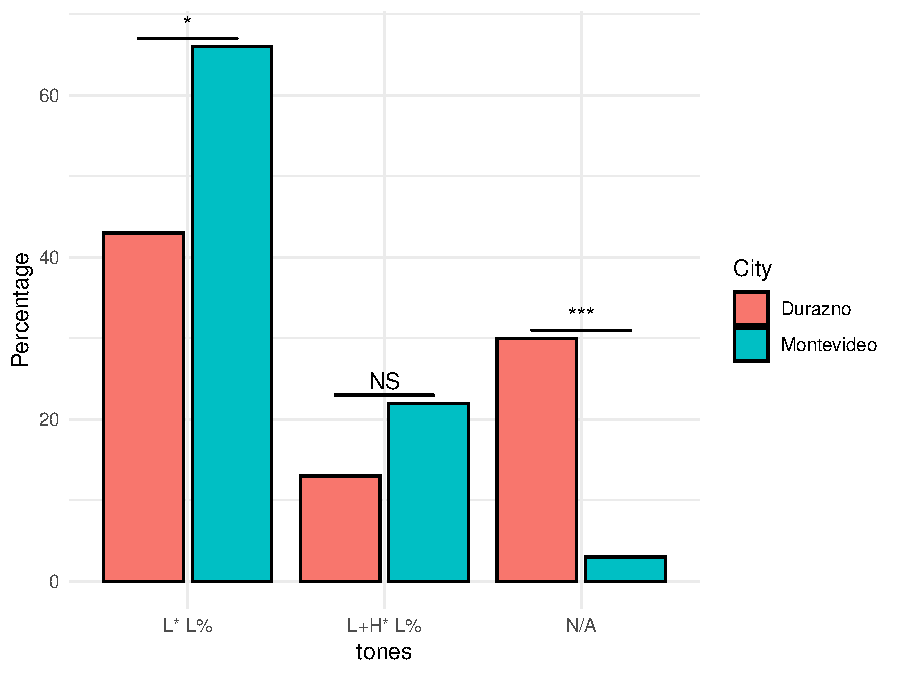
\includegraphics{main_files/figure-latex/unnamed-chunk-5-1.pdf}

\begin{quote}
In BFD we could mostly ignore boundary tones (e.g., L- and L\%)''
\end{quote}

We can integrate these if you prefer, but there does not look like there would be a major shift in the trend.

\emph{Narrow Focus Declaratives}

Full list, unchanged:

\begin{longtable}[]{@{}lrr@{}}
\caption{\label{tab:unnamed-chunk-6}Total percentage of each pitch accent in nuclear position for Narrow Focus Decaratives.}\tabularnewline
\toprule\noalign{}
tones & Montevideo & Durazno \\
\midrule\noalign{}
\endfirsthead
\toprule\noalign{}
tones & Montevideo & Durazno \\
\midrule\noalign{}
\endhead
\bottomrule\noalign{}
\endlastfoot
!H* L\% & 1 & 0 \\
H+L* L\% & 5 & 4 \\
L L\% & 1 & 0 \\
L* L\% & 25 & 28 \\
L+!H* L\% & 1 & 1 \\
L+!H*+L L\% & 2 & 2 \\
L+H* & 0 & 1 \\
L+H* !H\% & 3 & 12 \\
L+H* L\% & 23 & 32 \\
L+H* L\% & 1 & 0 \\
L+H*+L H\% & 1 & 0 \\
L+H*+L L\% & 17 & 3 \\
L+H*L\% & 0 & 1 \\
L+¡H L\% & 0 & 1 \\
L+¡H* !H\% & 1 & 1 \\
L+¡H* H\% & 0 & 1 \\
L+¡H* L\% & 13 & 7 \\
L+¡H*+L L\% & 4 & 1 \\
L+¡H*+L LH\% & 1 & 0 \\
L+¡H*L\% & 1 & 0 \\
¡H+L* L\% & 1 & 0 \\
NA & 1 & 5 \\
\end{longtable}

Full list, at least 5 total occurrences:

\begin{longtable}[]{@{}lrr@{}}
\caption{\label{tab:unnamed-chunk-7}Total percentage of each pitch accent in nuclear position in which one group had produced it atleast 5 percent of the time in the data for Narrow Focus Decaratives.}\tabularnewline
\toprule\noalign{}
tones & Montevideo & Durazno \\
\midrule\noalign{}
\endfirsthead
\toprule\noalign{}
tones & Montevideo & Durazno \\
\midrule\noalign{}
\endhead
\bottomrule\noalign{}
\endlastfoot
L* L\% & 25 & 28 \\
L+H* !H\% & 3 & 12 \\
L+H* L\% & 23 & 32 \\
L+H*+L L\% & 17 & 3 \\
L+¡H* L\% & 13 & 7 \\
\end{longtable}

\emph{Plot of Table 4}
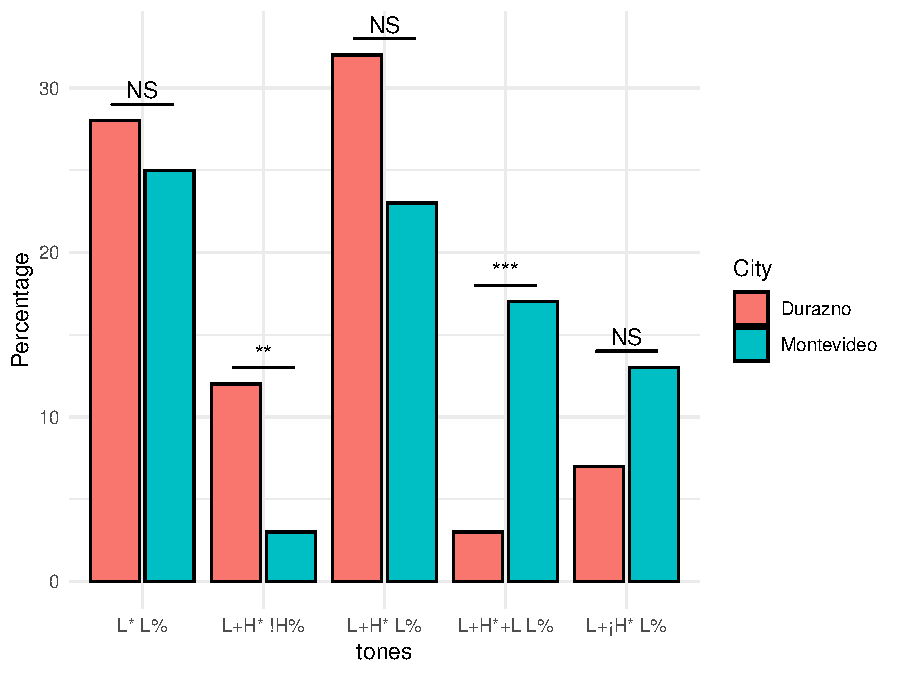
\includegraphics{main_files/figure-latex/unnamed-chunk-8-1.pdf}

\begin{quote}
In the NFD it becomes clear that the !H\% IP boundary tone is a clear difference between DZ (which has it) and MV (that mostly doesnt).''
\end{quote}

There is a significant difference here (p \textless{} .005).

\begin{quote}
At the same time we see that the tritonal L+H*+L is more common in MV than DZ.
\end{quote}

This is descriptively true (the count for MV is higher), but the poisson regression was not significant in this case (p \textgreater{} .05). This does not mean the difference is not real, but more likely that there just isn't enough data for the model to return a significant effect.

\begin{quote}
L*+H is more common in DZ than MV.
\end{quote}

I don't actually see this in the data.

\begin{quote}
What seems clear in both DZ and MV is that upstepping (¡) is a big part of marking focus, thus in an utterance full of L+H\emph{, focus is rightly marked with L+¡H}, in cases such as NFD5 Con Manuel, these are all high peaks but due to the lack of an earlier comparative peak they are not classified as upstepped.
\end{quote}

Here's a plot showing both cities productions for NFD5. It looks like the two groups are a little different than you've described above: Durazno speakers prefer L+H* !H\%.
The Montevideo group, on the other hand, produce L+H*+L L\%

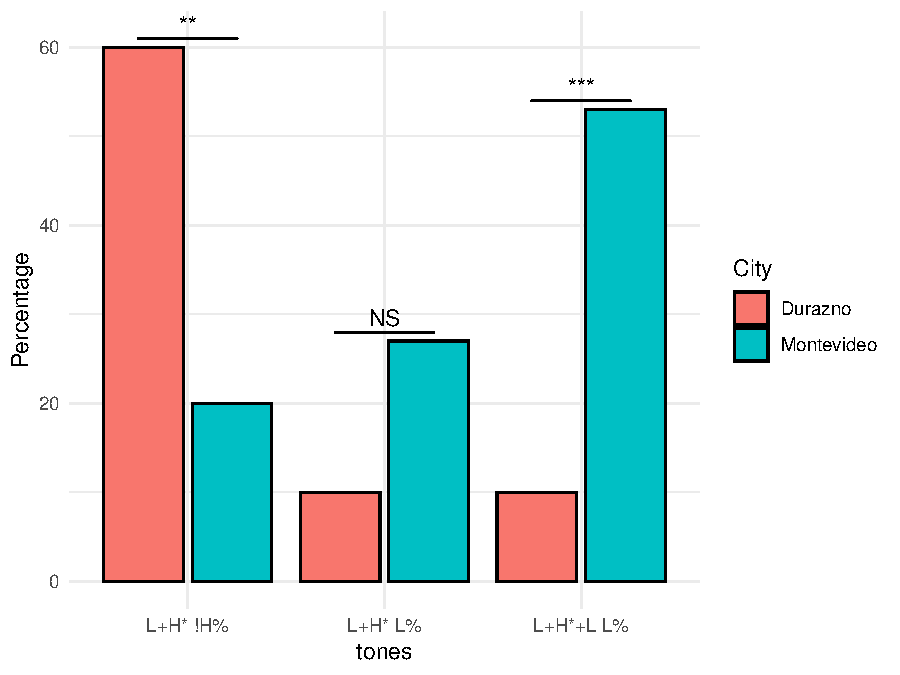
\includegraphics{main_files/figure-latex/unnamed-chunk-9-1.pdf}

\begin{quote}
Thus if in the count for focalized items L+H* rather than L+¡H* it should be undestood that these are, in such a case not different and can be grouped, whereas in sentences with PN peaks these are different.
\end{quote}

Let me know about specific groupings (a list would be ideal), and I can systematically integrate them in the analysis pipeline, which will spit out new plots etc. just by being run again after necessary adjustments.

\begin{quote}
Socially, (at least before the current updated data) women tended to use the tritonal L+H*+L as well as the upstep ¡ more than men, this again is a key distinction as it once again provided evidence for the theory of females making greater contrasts and therfore greater clarity in speaking.
\end{quote}

\begin{quote}
Also if you find that certain utterance tend to prefer unique forms, such as NFD5 ``a statement of the obvious'' where tritonals may be more common or where the mid-boundary tone !H\% is more frequent this is also of note.
\end{quote}


\end{document}
